
%\documentstyle[epsf,twocolumn]{jarticle}       %LaTeX2e仕様
% \documentclass[twocolumn]{jarticle}     %pLaTeX2e仕様(platex.exeの場合)
\documentclass[onecolumn]{ujarticle}   %pLaTeX2e仕様(uplatex.exeの場合)
%%%%%%%%%%%%%%%%%%%%%%%%%%%%%%%%%%%%%%%%%%%%%%%%%%%%%%%%%%%%%%
%%
%%  基本バージョン
%%
%%%%%%%%%%%%%%%%%%%%%%%%%%%%%%%%%%%%%%%%%%%%%%%%%%%%%%%%%%%%%%%%
\setlength{\topmargin}{-45pt}
%\setlength{\oddsidemargin}{0cm}
\setlength{\oddsidemargin}{-7.5mm}
%\setlength{\evensidemargin}{0cm}
\setlength{\textheight}{24.1cm}
%setlength{\textheight}{25cm}
\setlength{\textwidth}{17.4cm}
%\setlength{\textwidth}{172mm}
\setlength{\columnsep}{11mm}

%\kanjiskip=.07zw plus.5pt minus.5pt


% 【節が変わるごとに (1.1)(1.2) … (2.1)(2.2) と数式番号をつけるとき】
%\makeatletter
%\renewcommand{\theequation}{%
%\thesection.\arabic{equation}} %\@addtoreset{equation}{section}
%\makeatother

%\renewcommand{\arraystretch}{0.95} 行間の設定
%%%%%%%%%%%%%%%%%%%%%%%%%%%%%%%%%%%%%%%%%%%%%%%%%%%%%%%%
%\usepackage{graphicx}   %pLaTeX2e仕様(\documentstyle ->\documentclass)
\usepackage[dvipdfmx]{graphicx}
\usepackage{subcaption}
\usepackage{multirow}
\usepackage{amsmath}
\usepackage{url}
\usepackage{ulem}
\usepackage{algorithm}
\usepackage{algorithmic}
\usepackage{listings} %,jlisting} %日本語のコメントアウトをする場合jlistingが必要
%ここからソースコードの表示に関する設定
\lstset{
  basicstyle={\ttfamily},
  identifierstyle={\small},
  commentstyle={\smallitshape},
  keywordstyle={\small\bfseries},
  ndkeywordstyle={\small},
  stringstyle={\small\ttfamily},
  frame={tb},
  breaklines=true,
  columns=[l]{fullflexible},
  numbers=left,
  xrightmargin=0zw,
  xleftmargin=3zw,
  numberstyle={\scriptsize},
  stepnumber=1,
  numbersep=1zw,
  lineskip=-0.5ex
}
\newcommand{\argmax}{\mathop{\rm arg~max}\limits}
\newcommand{\argmin}{\mathop{\rm arg~min}\limits}

%%%%%%%%%%%%%%%%%%%%%%%%%%%%%%%%%%%%%%%%%%%%%%%%%%%%%%%%
\begin{document}

	%bibtex用の設定
	%\bibliographystyle{ujarticle}

	% \twocolumn[
		\noindent
		\hspace{1em}
		2022 年 6 月 10 日
		ゼミ資料
		\hfill
		杉山 竜弥
		\vspace{2mm}

		\hrule
		\begin{center}
			{\Large \bf 進捗報告}
		\end{center}
		\hrule
		\vspace{9mm}
	% ]


\section{今週やったこと}
\begin{itemize}
  \item スケッチデータの変換
\end{itemize}

\section{スケッチデータの変換}
スケッチを正順,逆順,シャッフル,分割など,描き順を変換できるようにした.

(変換後の順序は別資料のgifを参考にする)

今回は,逆順とシャッフルについてそれぞれ正順と再構築した結果を比較した.
逆順はほとんど復元できているものが少なく,直線で終わる結果が多かった.
おそらくスケッチの最後は目やしっぽなど,小さな特徴を描き足していく段階で,
内部のベクトルが飛び飛びになるものが RNN にとって難しいくデータも少ないため,
上手くいかなかったと考えられる.
最終的な状態は同じでもやはり内部の潜在変数は,大きく異るようである.

シャッフルでは場合によって,
オリジナルと比較すると復元できていると言えるものもあった.
元データは人間が書いたものなので,
逆順よりは人間に近い変換になりやすかったのだと考えられる.

\section{モデルの性能}
今回のモデルは手元で長時間訓練したものであったが,
性能に疑問が残った.

事前学習モデルをかなり探してみたが,
シングルクラスのものばかりで,
あまりいいモデルが見つからかなった.
もし本当ならば Sketch RNN の重大な欠陥であるが,
マルチクラスの学習が苦手であるという情報もあった.

\url{https://magenta.tensorflow.org/assets/sketch_rnn_demo/index.html}(デモページ)

実際デモの everything モデルで試すと,
それぞれのクラスで学習したモデルよりも,
結果が悪いと感じた.

このマルチクラスの問題をどうするか非常に悩んでいます.

\section{予定}
今回実験できなかった分割して潜在変数の和をとると,どのくらい復元されるのかをみたい.

% 7/6

\newpage
\begin{figure}[th]
  \begin{center}
    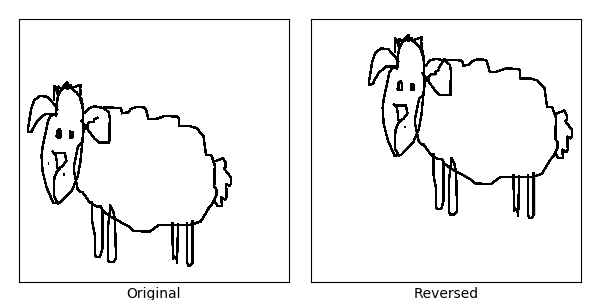
\includegraphics[clip,width=80mm]{sketch_tra_reverse_0.png}
    \caption{逆順スケッチ}
    \label{fig:result1}
  \end{center}
\end{figure}
\begin{figure}[th]
  \begin{center}
    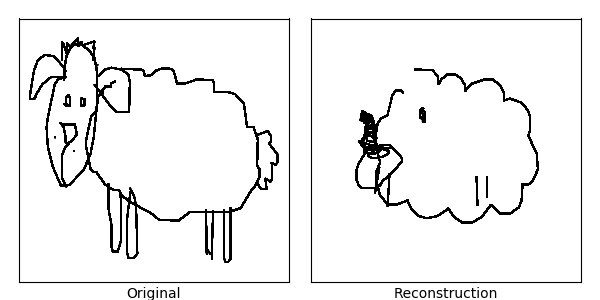
\includegraphics[clip,width=80mm]{sketch_tra_reverse_org_0.png}
    \caption{逆順スケッチ:オリジナル}
    \label{fig:result1_org}
  \end{center}
\end{figure}
\begin{figure}[th]
  \begin{center}
    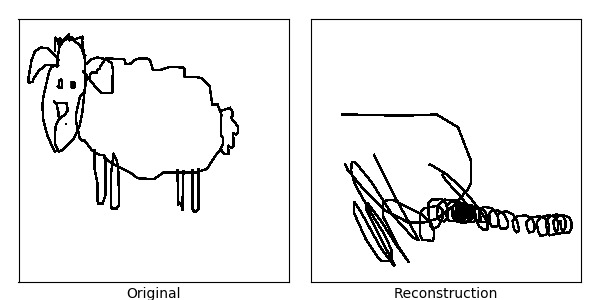
\includegraphics[clip,width=80mm]{sketch_tra_reverse_rvr_0.png}
    \caption{逆順スケッチ:変換後}
    \label{fig:result1_rvr}
  \end{center}
\end{figure}

\newpage
\begin{figure}[th]
  \begin{center}
    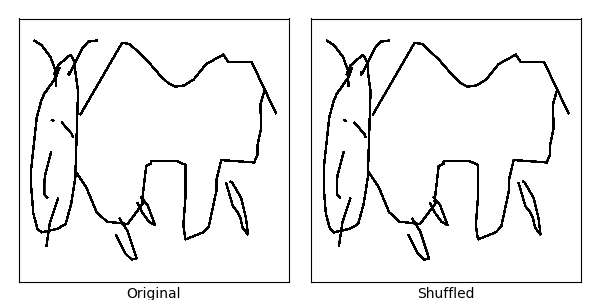
\includegraphics[clip,width=80mm]{sketch_tra_shuffle_0.png}
    \caption{シャッフルスケッチ}
    \label{fig:result2}
  \end{center}
\end{figure}
\begin{figure}[th]
  \begin{center}
    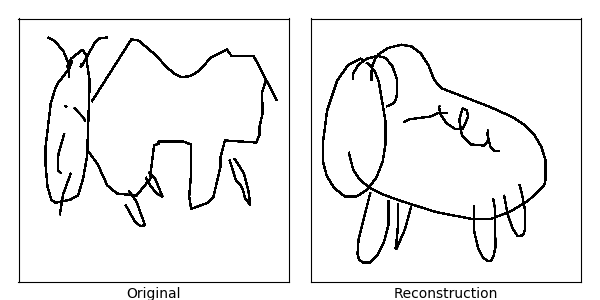
\includegraphics[clip,width=80mm]{sketch_tra_shuffle_org_0.png}
    \caption{シャッフルスケッチ:オリジナル}
    \label{fig:result2_org}
  \end{center}
\end{figure}
\begin{figure}[th]
  \begin{center}
    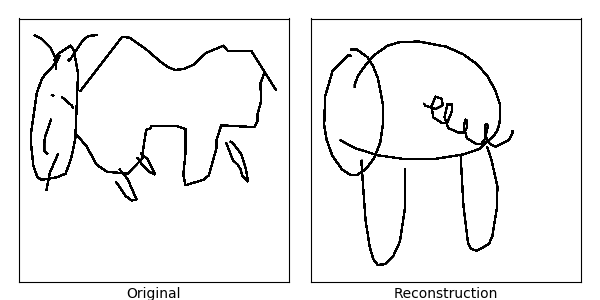
\includegraphics[clip,width=80mm]{sketch_tra_shuffle_rvr_0.png}
    \caption{シャッフルスケッチ:変換後}
    \label{fig:result2_rvr}
  \end{center}
\end{figure}



% \begin{figure}[th]
%   \begin{center}
%     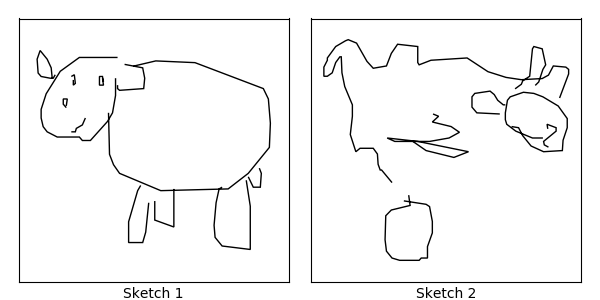
\includegraphics[clip,width=80mm]{compare.png}
%     \caption{別々のイラスト -0.09293087}
%     \label{fig:result1}
%   \end{center}
% \end{figure}





% 参考文献リスト
% \bibliographystyle{unsrt}
% \bibliography{ref}
\end{document}
